% ============================================================================
% Shared preamble for BOTH documents:
%   main.tex            -- the 8-page main-track paper
%   main_supplement.tex -- the separate supplementary PDF
%
% Kept in one file so theorem environments, notation macros, and title metadata
% cannot drift between the paper and its supplement. xr is loaded here (inert
% unless \externaldocument is called) so the supplement can resolve the ~57
% main-body cross-references it makes.
% ============================================================================
\documentclass[sigconf,anonymous]{aamas}

% ---- AAMAS 2027 IFAAMAS copyright block (do not change!) ----
\makeatletter
\gdef\@copyrightpermission{
  \begin{minipage}{0.2\columnwidth}
   \href{https://creativecommons.org/licenses/by/4.0/}{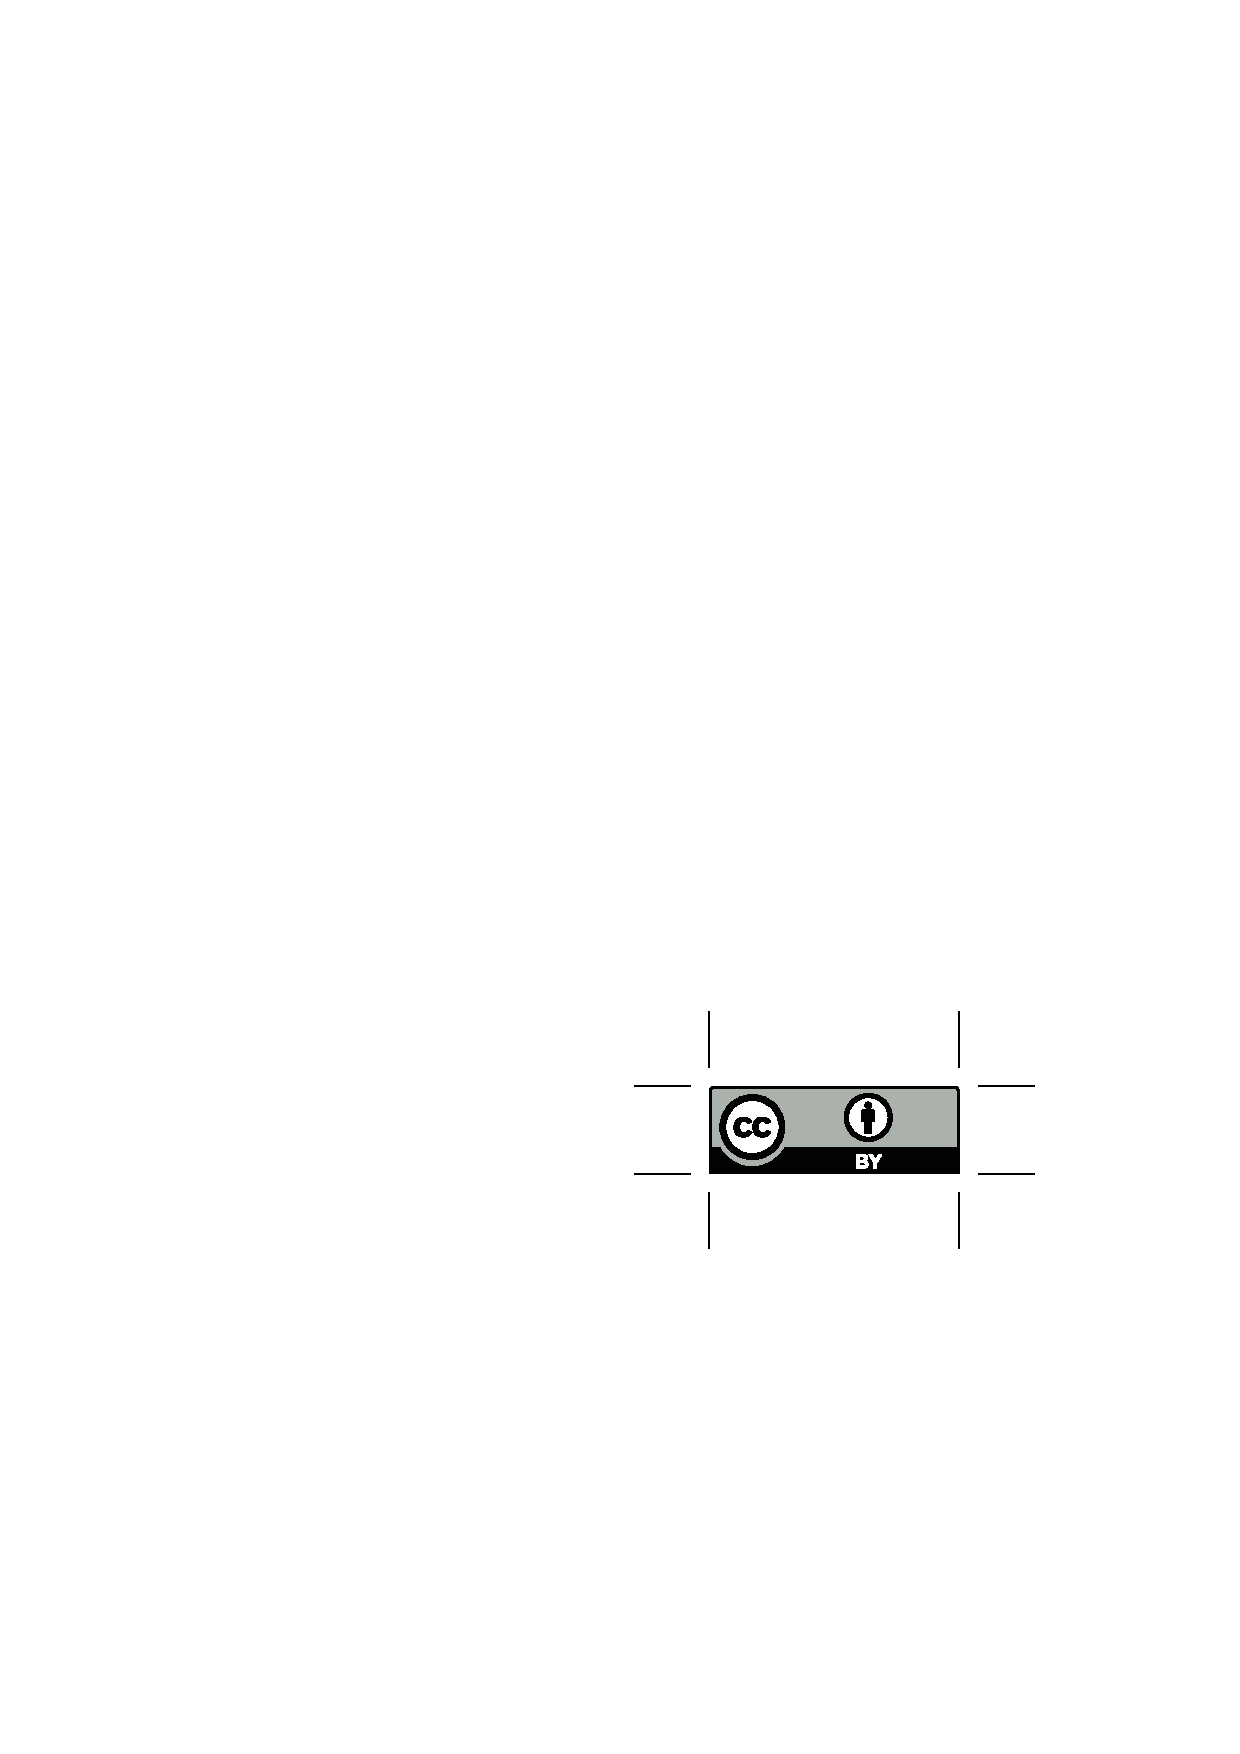
\includegraphics[width=0.90\textwidth]{by}}
  \end{minipage}\hfill
  \begin{minipage}{0.8\columnwidth}
   \href{https://creativecommons.org/licenses/by/4.0/}{This work is licensed under a Creative Commons Attribution International 4.0 License.}
  \end{minipage}
  \vspace{5pt}
}
\makeatother

\setcopyright{ifaamas}
\acmConference[AAMAS 2027]{Proc.\@ of the 26th International Conference
on Autonomous Agents and Multiagent Systems (AAMAS 2027)}{3--7 May 2027}{Hanoi, Vietnam}{M.~Baldoni, F.~Fang, W.~Yeoh, N.~Yorke-Smith (eds.)}
\copyrightyear{2027}
\acmYear{2027}
\acmDOI{}
\acmISBN{}
\acmSubmissionID{MASGym-2027-001}
\submissionType{Research Paper Track}

% ---- encoding / fonts ----
\usepackage[utf8]{inputenc}
\usepackage[T1]{fontenc}
\usepackage{microtype}
\usepackage{balance}

% ---- math ----
% NOTE: use amsfonts (not amssymb): acmart/sigconf loads newtxmath, and
% amssymb's \Bbbk redefinition conflicts with it.
\usepackage{amsmath,amsfonts,amsthm,mathtools,bm}
\usepackage{xspace}

% ---- citations (author--year, natbib is loaded by acmart) ----
\citestyle{acmauthoryear}

% ---- lists / tables / floats ----
\usepackage{enumitem}
\usepackage{booktabs,multirow,array}
\usepackage{xcolor}
\usepackage{float}

% ---- graphics: TikZ / PGFPlots ----
\usepackage{tikz}
\usetikzlibrary{arrows.meta,positioning,calc,fit,backgrounds,shapes.geometric,%
  shapes.symbols,decorations.pathreplacing,patterns,matrix,shadows.blur}
\usepackage{pgfplots}
\pgfplotsset{compat=1.18}
\usepgfplotslibrary{groupplots,fillbetween}

% ---- cross-document references (inert unless \externaldocument is used) ----
% Must be loaded before hyperref/cleveref resolve, hence its position here.
\usepackage{xr}

% ---- hyperlinks + clever references (hyperref is loaded by acmart) ----
\usepackage{cleveref}

% ---- shared TikZ styles (visual grammar) ----
% ============================================================================
% figures/tikz_styles.tex
% Shared visual grammar for all MASGym figures.
% Colour code (also encoded by shape/pattern for grayscale readability):
%   blue   = honest / normal system component (agents, orchestrator, memory)
%   orange/red = adversarial (colluders, compromised orchestrator, malicious tool, Sybil)
%   green  = defense / blue-team / deterministic checker (trusted evaluation)
%   purple = theory / mathematics
%   gray   = infrastructure / environment harness / background
% Arrow lanes: dataflow (blue), ctrlflow (gray dashed), advflow (red dashed),
%   defflow (green), theoryflow (purple).
% ============================================================================

% ---- palette ----
\definecolor{honest}{RGB}{31,97,164}      % blue
\definecolor{honestbg}{RGB}{219,232,246}
\definecolor{advers}{RGB}{200,63,42}      % red-orange
\definecolor{adversbg}{RGB}{250,224,216}
\definecolor{defense}{RGB}{34,139,80}     % green
\definecolor{defensebg}{RGB}{219,241,226}
\definecolor{theorycol}{RGB}{120,66,161}  % purple
\definecolor{theorybg}{RGB}{233,223,244}
\definecolor{infra}{RGB}{90,90,95}        % gray
\definecolor{infrabg}{RGB}{233,233,236}
\definecolor{amber}{RGB}{214,158,46}
\definecolor{amberbg}{RGB}{250,240,214}

% ---- generic node styles ----
\tikzset{
  >={Latex[length=2.4mm,width=1.8mm]},
  font=\small,
  block/.style={
    rounded corners=2pt, draw=infra!80, fill=infrabg, line width=0.7pt,
    align=center, inner sep=4pt, minimum height=8mm, text width=24mm},
  honestblock/.style={block, draw=honest!85, fill=honestbg, text=black},
  advblock/.style={block, draw=advers!85, fill=adversbg, text=black,
    dash pattern=on 3pt off 1.5pt},
  defblock/.style={block, draw=defense!80, fill=defensebg, text=black},
  theoryblock/.style={block, draw=theorycol!80, fill=theorybg, text=black},
  infrablock/.style={block, draw=infra!80, fill=infrabg},
  amberblock/.style={block, draw=amber!85, fill=amberbg, text=black},
  smalllabel/.style={font=\footnotesize, inner sep=1pt},
  arlbl/.style={midway, fill=white, inner sep=1.5pt, font=\scriptsize},
  % arrow "lanes"
  dataflow/.style={-{Latex[length=2.2mm]}, honest!85, line width=0.9pt},
  ctrlflow/.style={-{Latex[length=2.2mm]}, infra!85, line width=0.8pt,
    densely dashed},
  advflow/.style={-{Latex[length=2.2mm]}, advers!85, line width=1.0pt,
    dash pattern=on 3pt off 1.6pt},
  defflow/.style={-{Latex[length=2.2mm]}, defense!80, line width=1.0pt},
  theoryflow/.style={-{Latex[length=2.2mm]}, theorycol!80, line width=0.9pt},
  grp/.style={rounded corners=4pt, draw=#1!55, line width=0.8pt,
    fill=#1!5, inner sep=6pt},
  grp/.default=infra,
}

% ============================================================================
% Pure-TikZ icons (no external images, no fontawesome dependency).
% Each is a "pic" scaled to ~6mm; call with:  \pic at (x,y) {agenticon};
% ============================================================================

% -- worker agent (rounded robot head) --
\tikzset{
  agenticon/.pic={
    \draw[honest!85, fill=honestbg, line width=0.7pt, rounded corners=1pt]
      (-2.6mm,-2.2mm) rectangle (2.6mm,2.4mm);
    \draw[honest!85, fill=white, line width=0.5pt] (-1.2mm,0.3mm) circle (0.7mm);
    \draw[honest!85, fill=white, line width=0.5pt] (1.2mm,0.3mm) circle (0.7mm);
    \draw[honest!85, line width=0.6pt] (-1mm,-1.3mm) -- (1mm,-1.3mm);
    \draw[honest!85, line width=0.6pt] (0,2.4mm) -- (0,3.4mm);
    \fill[honest!85] (0,3.5mm) circle (0.5mm);
  }
}

% -- orchestrator (hub with crown) --
\tikzset{
  orchicon/.pic={
    \draw[honest!90, fill=honestbg, line width=0.8pt] (0,0) circle (2.7mm);
    \draw[honest!90, fill=honest!25, line width=0.6pt]
      (-2mm,0.6mm)--(-1mm,2.2mm)--(0,0.9mm)--(1mm,2.2mm)--(2mm,0.6mm)--(2mm,-0.4mm)--(-2mm,-0.4mm)--cycle;
    \fill[honest!90] (-2mm,0.6mm) circle (0.35mm);
    \fill[honest!90] (0,0.9mm) circle (0.35mm);
    \fill[honest!90] (2mm,0.6mm) circle (0.35mm);
  }
}

% -- compromised orchestrator (hub with crown + cross) --
\tikzset{
  orchbadicon/.pic={
    \draw[advers!90, fill=adversbg, line width=0.8pt] (0,0) circle (2.7mm);
    \draw[advers!90, fill=advers!20, line width=0.6pt]
      (-2mm,0.6mm)--(-1mm,2.2mm)--(0,0.9mm)--(1mm,2.2mm)--(2mm,0.6mm)--(2mm,-0.4mm)--(-2mm,-0.4mm)--cycle;
    \draw[advers!95, line width=0.9pt] (-1.2mm,-1.0mm)--(1.2mm,-2.4mm);
    \draw[advers!95, line width=0.9pt] (-1.2mm,-2.4mm)--(1.2mm,-1.0mm);
  }
}

% -- Byzantine / attacker node (warning cross) --
\tikzset{
  attackericon/.pic={
    \draw[advers!90, fill=adversbg, line width=0.8pt] (0,0) circle (2.7mm);
    \draw[advers!90, line width=0.9pt] (-1.3mm,-1.3mm)--(1.3mm,1.3mm);
    \draw[advers!90, line width=0.9pt] (-1.3mm,1.3mm)--(1.3mm,-1.3mm);
  }
}

% -- Sybil (two overlapping identity disks) --
\tikzset{
  sybilicon/.pic={
    \draw[advers!85, fill=adversbg, line width=0.7pt] (-1.1mm,0) circle (2.0mm);
    \draw[advers!85, fill=adversbg, line width=0.7pt] (1.1mm,0) circle (2.0mm);
    \draw[advers!85, line width=0.6pt] (-1.1mm,-0.4mm) circle (0.6mm);
    \draw[advers!85, line width=0.6pt] (1.1mm,-0.4mm) circle (0.6mm);
  }
}

% -- shield (defense / blue team) --
\tikzset{
  shieldicon/.pic={
    \draw[defense!85, fill=defensebg, line width=0.8pt]
      (0,3mm) -- (2.4mm,1.6mm) -- (2.4mm,-1mm) -- (0,-3mm)
      -- (-2.4mm,-1mm) -- (-2.4mm,1.6mm) -- cycle;
    \draw[defense!85, line width=0.9pt] (-1.1mm,0.2mm)--(-0.2mm,-1.2mm)--(1.4mm,1.2mm);
  }
}

% -- deterministic checker (clipboard + tick) --
\tikzset{
  checkericon/.pic={
    \draw[defense!85, fill=defensebg, line width=0.7pt, rounded corners=0.6pt]
      (-2mm,-2.7mm) rectangle (2mm,2.7mm);
    \draw[defense!85, fill=white, line width=0.5pt] (-0.9mm,2.3mm) rectangle (0.9mm,3.1mm);
    \draw[defense!85, line width=0.9pt] (-1.2mm,0.2mm)--(-0.3mm,-1.0mm)--(1.4mm,1.4mm);
  }
}

% -- LM tool emulator (cloud with function symbol) --
\tikzset{
  emuicon/.pic={
    \draw[infra!85, fill=infrabg, line width=0.7pt]
      (-2.4mm,-0.6mm) .. controls (-2.8mm,1.4mm) and (-0.9mm,1.9mm) .. (-0.6mm,1.2mm)
      .. controls (0.0mm,2.3mm) and (1.6mm,2.0mm) .. (1.5mm,0.9mm)
      .. controls (2.6mm,0.9mm) and (2.5mm,-0.8mm) .. (1.4mm,-0.9mm)
      -- (-2.0mm,-0.9mm) .. controls (-2.6mm,-0.9mm) and (-2.6mm,-0.6mm) .. (-2.4mm,-0.6mm) -- cycle;
    \node[infra!90, font=\scriptsize\itshape] at (0,0.1mm) {f};
  }
}

% -- tool (gear) --
\tikzset{
  toolicon/.pic={
    \draw[infra!85, fill=infrabg, line width=0.7pt] (0,0) circle (1.9mm);
    \foreach \a in {0,45,...,315}{
      \draw[infra!85, line width=0.8pt] (\a:1.9mm)--(\a:2.8mm);}
    \draw[infra!85, fill=white, line width=0.5pt] (0,0) circle (0.7mm);
  }
}

% -- malicious tool (gear, red, with cross) --
\tikzset{
  toolbadicon/.pic={
    \draw[advers!85, fill=adversbg, line width=0.7pt] (0,0) circle (1.9mm);
    \foreach \a in {0,45,...,315}{
      \draw[advers!85, line width=0.8pt] (\a:1.9mm)--(\a:2.8mm);}
    \draw[advers!90, line width=0.8pt] (-0.9mm,-0.9mm)--(0.9mm,0.9mm);
    \draw[advers!90, line width=0.8pt] (-0.9mm,0.9mm)--(0.9mm,-0.9mm);
  }
}

% -- shared memory store (cylinder/stack) --
\tikzset{
  memicon/.pic={
    \draw[honest!85, fill=honestbg, line width=0.7pt]
      (-2mm,-2.4mm) -- (-2mm,2mm) arc (180:0:2mm and 0.7mm) -- (2mm,-2.4mm)
      arc (0:-180:2mm and 0.7mm);
    \draw[honest!85, line width=0.6pt] (-2mm,2mm) arc (180:360:2mm and 0.7mm);
    \draw[honest!85, line width=0.5pt] (-2mm,0.4mm) arc (180:360:2mm and 0.7mm);
    \draw[honest!85, line width=0.5pt] (-2mm,-1.2mm) arc (180:360:2mm and 0.7mm);
  }
}

% -- poisoned memory (cylinder, red, droplet) --
\tikzset{
  membadicon/.pic={
    \draw[advers!85, fill=adversbg, line width=0.7pt]
      (-2mm,-2.4mm) -- (-2mm,2mm) arc (180:0:2mm and 0.7mm) -- (2mm,-2.4mm)
      arc (0:-180:2mm and 0.7mm);
    \draw[advers!85, line width=0.6pt] (-2mm,2mm) arc (180:360:2mm and 0.7mm);
    \fill[advers!80] (0,-0.2mm) circle (0.55mm);
  }
}

% -- neural net / model --
\tikzset{
  modelicon/.pic={
    \foreach \y in {-1.8mm,0mm,1.8mm}{\fill[honest!80] (-2.2mm,\y) circle (0.5mm);}
    \foreach \y in {-1mm,1mm}{\fill[honest!80] (0,\y) circle (0.5mm);}
    \fill[honest!80] (2.2mm,0) circle (0.5mm);
    \foreach \y in {-1.8mm,0mm,1.8mm}{\foreach \z in {-1mm,1mm}{
      \draw[honest!45, line width=0.3pt] (-2.2mm,\y)--(0,\z);}}
    \foreach \z in {-1mm,1mm}{\draw[honest!45, line width=0.3pt] (0,\z)--(2.2mm,0);}
  }
}

% -- database / dataset --
\tikzset{
  dbicon/.pic={
    \draw[infra!85, fill=infrabg, line width=0.7pt] (-2mm,-2.4mm) rectangle (2mm,2.4mm);
    \draw[infra!85, line width=0.6pt] (-2mm,1.2mm)--(2mm,1.2mm);
    \draw[infra!85, line width=0.6pt] (-2mm,0mm)--(2mm,0mm);
    \draw[infra!85, line width=0.6pt] (-2mm,-1.2mm)--(2mm,-1.2mm);
  }
}

% -- theorem scroll --
\tikzset{
  theoremicon/.pic={
    \draw[theorycol!80, fill=theorybg, line width=0.7pt, rounded corners=1pt]
      (-2mm,-2.6mm) rectangle (2mm,2.6mm);
    \draw[theorycol!80, line width=0.6pt] (-1.2mm,1.4mm)--(1.2mm,1.4mm);
    \draw[theorycol!80, line width=0.6pt] (-1.2mm,0.4mm)--(1.2mm,0.4mm);
    \draw[theorycol!80, line width=0.6pt] (-1.2mm,-0.6mm)--(0.6mm,-0.6mm);
  }
}

% -- human oversight (person) --
\tikzset{
  humanicon/.pic={
    \draw[infra!90, fill=infrabg, line width=0.7pt] (0,1.6mm) circle (1.0mm);
    \draw[infra!90, fill=infrabg, line width=0.7pt]
      (-1.6mm,-2.6mm) .. controls (-1.6mm,0.2mm) and (1.6mm,0.2mm) .. (1.6mm,-2.6mm) -- cycle;
  }
}

% ---- legend helper ----
\newcommand{\legendline}[2]{% #1 style, #2 text
  \draw[#1] (0,0) -- (5mm,0); \node[right, font=\scriptsize] at (5.5mm,0) {#2};}


% ============================================================================
% Theorem environments
% ============================================================================
\theoremstyle{plain}
\newtheorem{theorem}{Theorem}[section]
\newtheorem{lemma}[theorem]{Lemma}
\newtheorem{proposition}[theorem]{Proposition}
\newtheorem{corollary}[theorem]{Corollary}
\theoremstyle{definition}
\newtheorem{definition}[theorem]{Definition}
\newtheorem{assumption}{Assumption}
\theoremstyle{remark}
\newtheorem{remark}[theorem]{Remark}

\crefname{assumption}{Assumption}{Assumptions}
\Crefname{assumption}{Assumption}{Assumptions}

% ============================================================================
% Lightweight algorithm float + pseudocode macros
% (reproduce a numbered, ruled pseudocode listing with float.sty only)
% ============================================================================
\floatstyle{ruled}
\newfloat{algorithm}{tbp}{loa}
\floatname{algorithm}{Algorithm}
\crefname{algorithm}{Algorithm}{Algorithms}
\Crefname{algorithm}{Algorithm}{Algorithms}
\newcounter{algline}
\newlength{\algind}
\newcommand{\algreset}{\setcounter{algline}{0}\setlength{\algind}{0pt}}
\newcommand{\PL}[1]{\par\refstepcounter{algline}\noindent
  \makebox[2.6em][r]{\scriptsize\thealgline:\,}\hspace{0.5em}\hspace{\algind}%
  \ignorespaces#1\strut}
\newcommand{\Ind}{\addtolength{\algind}{1.5em}}
\newcommand{\Ded}{\addtolength{\algind}{-1.5em}}
\newcommand{\kw}[1]{\textbf{#1}}
\newcommand{\comm}[1]{\hfill{\footnotesize\itshape\color{black!55}\(\triangleright\)~#1}}

% ============================================================================
% Notation macros
% ============================================================================
\newcommand{\R}{\mathbb{R}}
\newcommand{\N}{\mathbb{N}}
\newcommand{\E}{\mathbb{E}}
\newcommand{\Prob}{\mathbb{P}}
\newcommand{\indic}{\mathbb{1}}
\newcommand{\Agents}{\mathcal{A}}          % set of agents
\newcommand{\Roles}{\mathcal{R}}           % role set
\newcommand{\Gtop}{\mathcal{G}}            % topology graph
\newcommand{\Vtop}{\mathcal{V}}
\newcommand{\Etop}{\mathcal{E}}
\newcommand{\Nin}{\mathcal{N}^{-}}          % inbound neighbourhood
\newcommand{\Trace}{\tau}                  % global state trace
\newcommand{\TraceSp}{\mathcal{T}}         % trace space
\newcommand{\Statesp}{\mathcal{S}}         % state space
\newcommand{\Predsec}{\Phi}                % system-level security predicate
\newcommand{\Predutil}{\Psi}               % benign-success predicate
\newcommand{\Checker}{\mathsf{C}}          % deterministic checker
\newcommand{\Emu}{\mathcal{E}_{\mathrm{LM}}} % LM tool emulator
\newcommand{\Judge}{\mathsf{J}}            % LLM judge (contrast)
\newcommand{\Advset}{\mathcal{B}}          % adversarial agent set
\newcommand{\betafrac}{\beta}              % adversary fraction
\newcommand{\config}{c}                    % environment configuration
\newcommand{\Configs}{\mathcal{C}}         % configuration space
\newcommand{\ASRs}{\mathrm{ASR}_{\mathrm{sys}}}
\newcommand{\ASRa}{\mathrm{ASR}_{\mathrm{act}}}
\newcommand{\PNAs}{\mathrm{PNA}_{\mathrm{sys}}}
\newcommand{\NRPs}{\mathrm{NRP}_{\mathrm{sys}}}
\newcommand{\CPR}{\mathrm{CPR}}            % compromise-propagation rate
\newcommand{\CSR}{\mathrm{CSR}}            % collusion success rate
\newcommand{\red}{\rho}                    % red policy
\newcommand{\blue}{\delta}                 % blue policy (defense)
\newcommand{\pinf}{p}                      % per-edge propagation probability
\newcommand{\thresh}{\theta}               % threshold (bootstrap percolation)
\newcommand{\kappaem}{\kappa}              % emulation agreement
\newcommand{\defname}{\textsc{MASGym}\xspace}
\newcommand{\corb}{\textsc{CoRB}\xspace}

% ============================================================================
% Title and author metadata (in the preamble, as in the official sample)
% ============================================================================
\title[MASGym: A Security Gym for Multi-Agent LLM Systems]{\defname: A
Co-Evolving Red/Blue Security Gym for Multi-Agent LLM Systems with
Parameterized Collusion, Orchestrator Compromise, and System-Level Metrics}

% Anonymous double-blind submission: the author block is suppressed by the
% `anonymous' class option. For camera-ready, remove that option and fill in
% your full author list, affiliations, and emails.
\author{Thanh Pham}
\affiliation{%
  \institution{School of Computing Technologies, RMIT University}
  \country{Melbourne, Australia}}
\email{thanhphamchivn@gmail.com}

% Abstract and keywords must be defined in the preamble, before \maketitle.
\begin{abstract}
Security research on large language model (LLM) agents is bottlenecked by its
instruments: the strongest existing benchmarks---Agent Security Bench (ASB),
AgentDojo, InjecAgent, and the ToolEmu sandbox---are single-agent. Yet deployed
systems are increasingly orchestrated \emph{collectives} in which a planner directs
workers, agents share memory, tools are third-party, and coordination is forced.
The phenomena that dominate risk in that regime---collusion, a compromised
orchestrator, malicious tools, Sybils, and group-level emergent failure---cannot be
produced, let alone measured, by a single-agent harness. We present \defname{}, an
environment and evaluation methodology purpose-built for multi-agent LLM security.
It contributes: (i) a forced-coordination task suite with heterogeneous roles,
partial observability, and system-level compromise objectives over star, chain,
tree, and mesh topologies at $3$--$50$ agents; (ii) a natively parameterized
adversary model (adversary fraction, collusion, adaptivity, orchestrator
compromise, malicious tools, Sybils, poisoned memory); (iii) a system-level metric
suite, $\NRPs=\PNAs(1-\ASRs)$, scored by a deterministic checker over the global
state trace---never an LLM judge on the critical path; and (iv) \corb, a
co-evolving red/blue protocol logging attack--defense trajectories and their
system-level scores. Supporting theory (proved under explicit assumptions):
an axiomatic characterization of the metric that reduces to ASB at one agent, an
evaluator-integrity theorem, topology-dependent compromise-propagation bounds, a
strict collusion advantage, a forced-coordination lower bound, and finite-sample
concentration. On a transparent, clearly-labelled \emph{synthetic} emulator, the
headline claim is measured: a per-agent guardrail's relative ASR reduction over
no-defense shrinks $41.6\%\to31.8\%\to27.6\%$ from the single-agent to the
collusion to the compromised-orchestrator context (Table~\ref{tab:degradation}).
\end{abstract}

\keywords{multi-agent LLM security; security benchmark and environment;
co-evolving red/blue evaluation; collusion; compromised orchestrator; Sybil attack;
prompt injection; tool emulation; deterministic security checking; system-level
metrics; compromise propagation}
